%!TEX root = ../../book_ML.tex
\chapter{Thiết kế và xây dựng hệ thống}
\label{cha:chap3}
% \index{principal component analysis}
% \index{PCA -- \textit{xem} principle component analysis}
% \index{PCA}

% \index{phân tích thành phần chính -- principle component analysis}
% \index{principle component analysis -- phân tích thành phần chính}
% \index{PCA}
\section{Phân tích}
Về cơ bản một hệ thống điểm danh bằng khuôn mặt gồm các bước sau:
\begin{itemize}
    \item Thu thập dữ liệu khuôn mặt
    \item Phát hiện khuôn mặt dựa trên ảnh đầu vào và gán nhãn dữ liệu
    \item Làm giàu dữ liệu
    \item Trích xuất các đặc trưng (sử dụng học sâu)
    \item Đưa các đặc trưng đã được gán nhãn vào thuật toán phân loại
    \item Lưu trữ các thông tin và kết quả phân loại đã được học
    \item Nhận dạng khuôn mặt và tiến hành điểm danh
\end{itemize}

Hệ thống được chia thành 2 quy trình:
\begin{itemize}
    \item Người dùng đăng ký khuôn mặt của mình
    \item Hệ thống tíến hành nhận dạng và điểm danh
\end{itemize}

\begin{figure}
    \begin{subfigure}{1.\textwidth}
        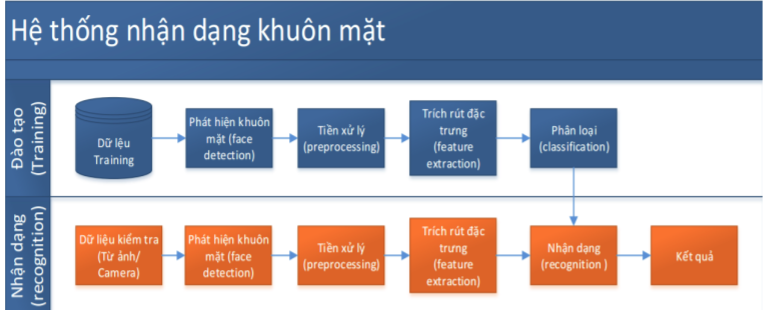
\includegraphics[width=1.\linewidth]{Chapters/items/chap3_1.jpg}
        \label{fig:chap3_1}
    \end{subfigure}
    \caption{Tổng quan hệ thống}
\end{figure}


\section{Xây dựng}

\subsection{Thu thập dữ liệu khuôn mặt}
Hệ thống thu thập hình ảnh dữ liệu khuôn mặt bằng cách sử dụng chính webcam
của máy tính, hoặc có thể là hình ảnh từ nhiều nguồn khác.
Các ảnh được thu thập cần đảm bảo các yếu tố như điều kiện ánh sáng,
các góc độc khác nhau của khuôn mặt, tuổi tác,…
Và khuôn mặt không nên có các vật cản như kính.

Hệ thống có thể gợi ý người dùng quay mặt sang trái hay phải để có thể thu thập được
nhiều góc mặt nhất có thể

\begin{figure}
    \begin{subfigure}{0.6\textwidth}
        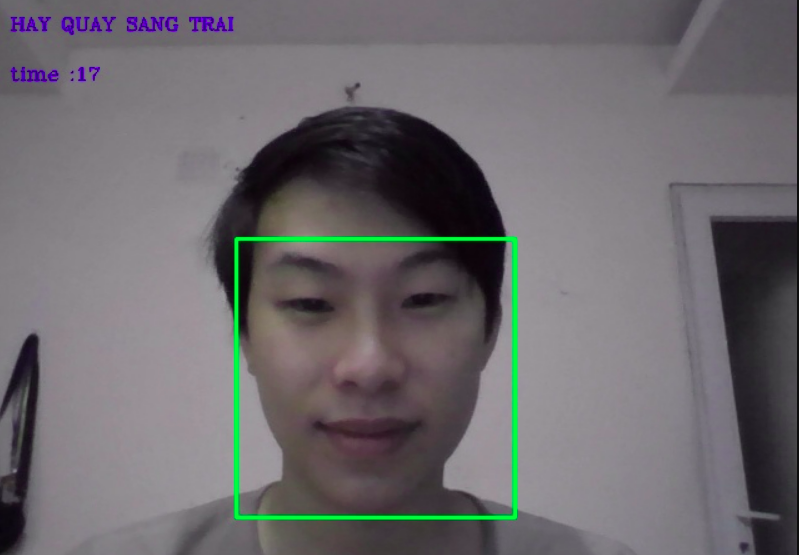
\includegraphics[width=1\linewidth]{Chapters/items/chap3_2.jpg}
        \label{fig:chap3_2}
    \end{subfigure}
    \caption{Thu thập dữ liệu khuôn mặt người dùng}
\end{figure}

\newpage
Ngoài ra, để đảm bảo độ chính xác cho hệ thống, đối với mỗi người dùng
cần thu thập một số lượng ảnh nhất định không quá ít, và mỗi bức ảnh chỉ
chứa duy nhất một khuôn mặt.

Bộ dữ liệu tôi sử dụng trong dự án này gồm 400 ảnh của 10 sinh viên.
Với số lượng ảnh của mỗi sinh viên là khác nhau dao động từ 30 đến 40
ảnh cho mỗi sinh viên.

\subsection{Phát hiện khuôn mặt và gán nhãn dữ liệu}
Để trích chọn đặc trưng cho mỗi khuôn mặt, trước tiên ta cần tìm ra
vị trí khuôn mặt trong bức hình. Vì bộ dữ liệu sẽ bao gồm nhiều ảnh
có điều kiện ánh sáng cũng như các góc độ của khuôn mặt khác nhau,
chính vì vậy việc lựa chọn máy dò khuôn mặt cũng rất quan trọng để đảm
hiệu quả cao nhất cho hệ thống.

Tôi sử dụng MTCNN thực hiện công việc này và tiến hành gán nhãn dữ liệu,
yêu cầu người dùng nhập tên.

\begin{figure}
    \begin{subfigure}{0.6\textwidth}
        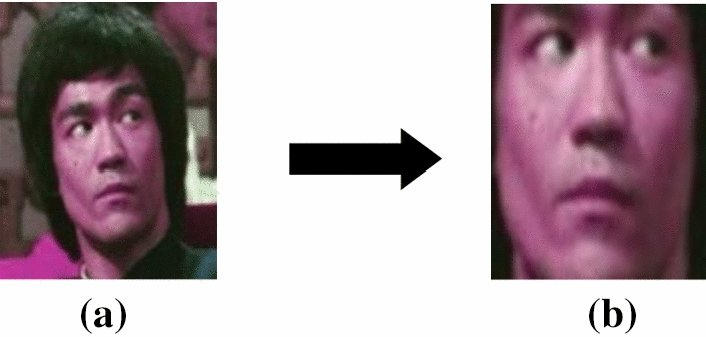
\includegraphics[width=1\linewidth]{Chapters/items/chap3_3.jpg}
        \label{fig:chap3_3}
    \end{subfigure}
    \caption{MTCNN lấy khuôn mặt của người dùng}
\end{figure}

\subsection{Làm giàu dữ liệu}

Dữ liệu là nguồn sống của học máy và học sâu, nhận thấy sự quan trọng của dữ liệu
trong các mô hình học sâu nên các phương pháp làm giàu dữ liệu đã ra đời và đóng góp rất nhiều
vào sự thành công của các mô hình học sâu.

Ở trong dự án này tôi cũng sử dụng một số phương pháp làm giàu dữ liệu phổ biến sử dụng các thuật toán xử lý ảnh:
\begin{itemize}
    \item Chuẩn hóa theo phân phối chuẩn các pixels của ảnh
    \item Tạo ảnh với các góc nghiêng 20 độ
    \item Dịch chuyển ảnh theo chiều dài và chiều rộng
    \item Lật ảnh theo chiều ngang
\end{itemize}

\begin{figure}
    \begin{subfigure}{1\textwidth}
        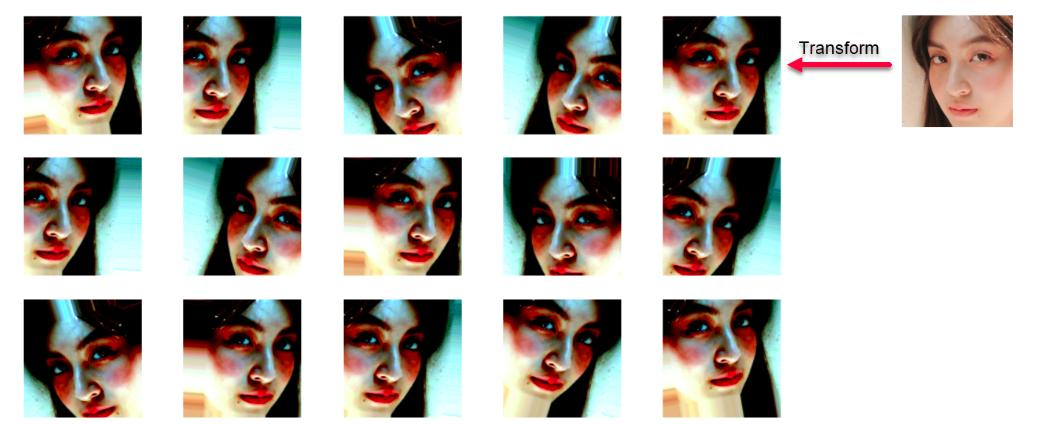
\includegraphics[width=1\linewidth]{Chapters/items/chap3_4.jpg}
        \label{fig:chap3_4}
    \end{subfigure}
    \caption{Dữ liệu đã đươc làm giàu}
\end{figure}

\subsection{Trích chọn các đặc trưng ảnh khuôn mặt}
Trong hệ thống này tôi sử dụng 1 mô hình có sẵn với mạng cơ sở là InceptionResnetV1 được
huẩn luyện trong tập dữ liệu với hàng triệu ảnh khuôn mặt khác nhau trong đó có cả người Việt Nam.

\begin{figure}
    \begin{subfigure}{0.4\textwidth}
        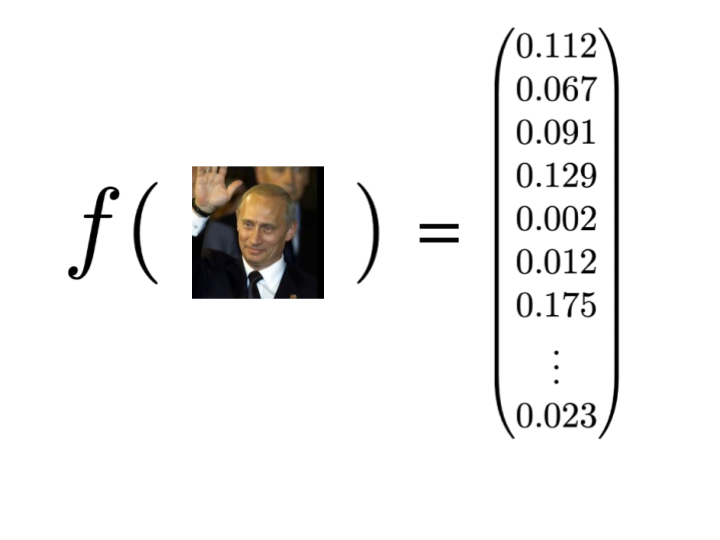
\includegraphics[width=1\linewidth]{Chapters/items/embed.png}
        \label{fig:embed}
    \end{subfigure}
    \caption{Mô tả nhúng ảnh khuôn mặt thành các vector đặc trưng}
\end{figure}

Bộ dữ liệu khuôn mặt sẽ được chia theo từng thư mục tương ứng với hình ảnh
của từng đối tượng (sinh viên). Hệ thống sẽ tiến hành quét qua toàn bộ ảnh
trong các thư mục. máy dò khuôn mặt sẽ tìm kiếm khuôn mặt có
trong ảnh (mặc định mỗi ảnh sẽ chỉ chưa một khuôn mặt),
cắt lấy khuôn mặt và đưa kích thước về 160x160 pixel.




Sau đó FaceNet sẽ tiến hành trích rút đặc trưng của từng khuôn mặt,
áp dụng mô hình học với thuật toán hàm đánh giá bộ ba và gắn nhãn cho từng
khuôn mặt (nhãn sẽ được lấy theo tên thư mục chứa ảnh).

\subsection{Đưa các vector đặc trưng vào mô hình phân loại}
Sau khi đã có các vector đặc trưng của các khuôn mặt, tôi sẽ đưa các vector này
vào một mô hình để thuật toán có thể học được cách phân loại các đối tượng đã đăng ký.

Mô hình thuât toán phân loại mà tôi sử dụng là thuật toán SVM (Support vector machine)

Sau khi thuât toán SVM đã được huấn luyện để phân loại xong thì tiến hành lưu kết quả huấn luyện cùng
với các vector và nhãn đã đào tạo lại, nhằm mục đích huẩn luyện lại mô hình khi có thêm khuôn mặt mới
đăng ký.

\begin{figure}
    \begin{subfigure}{0.8\textwidth}
        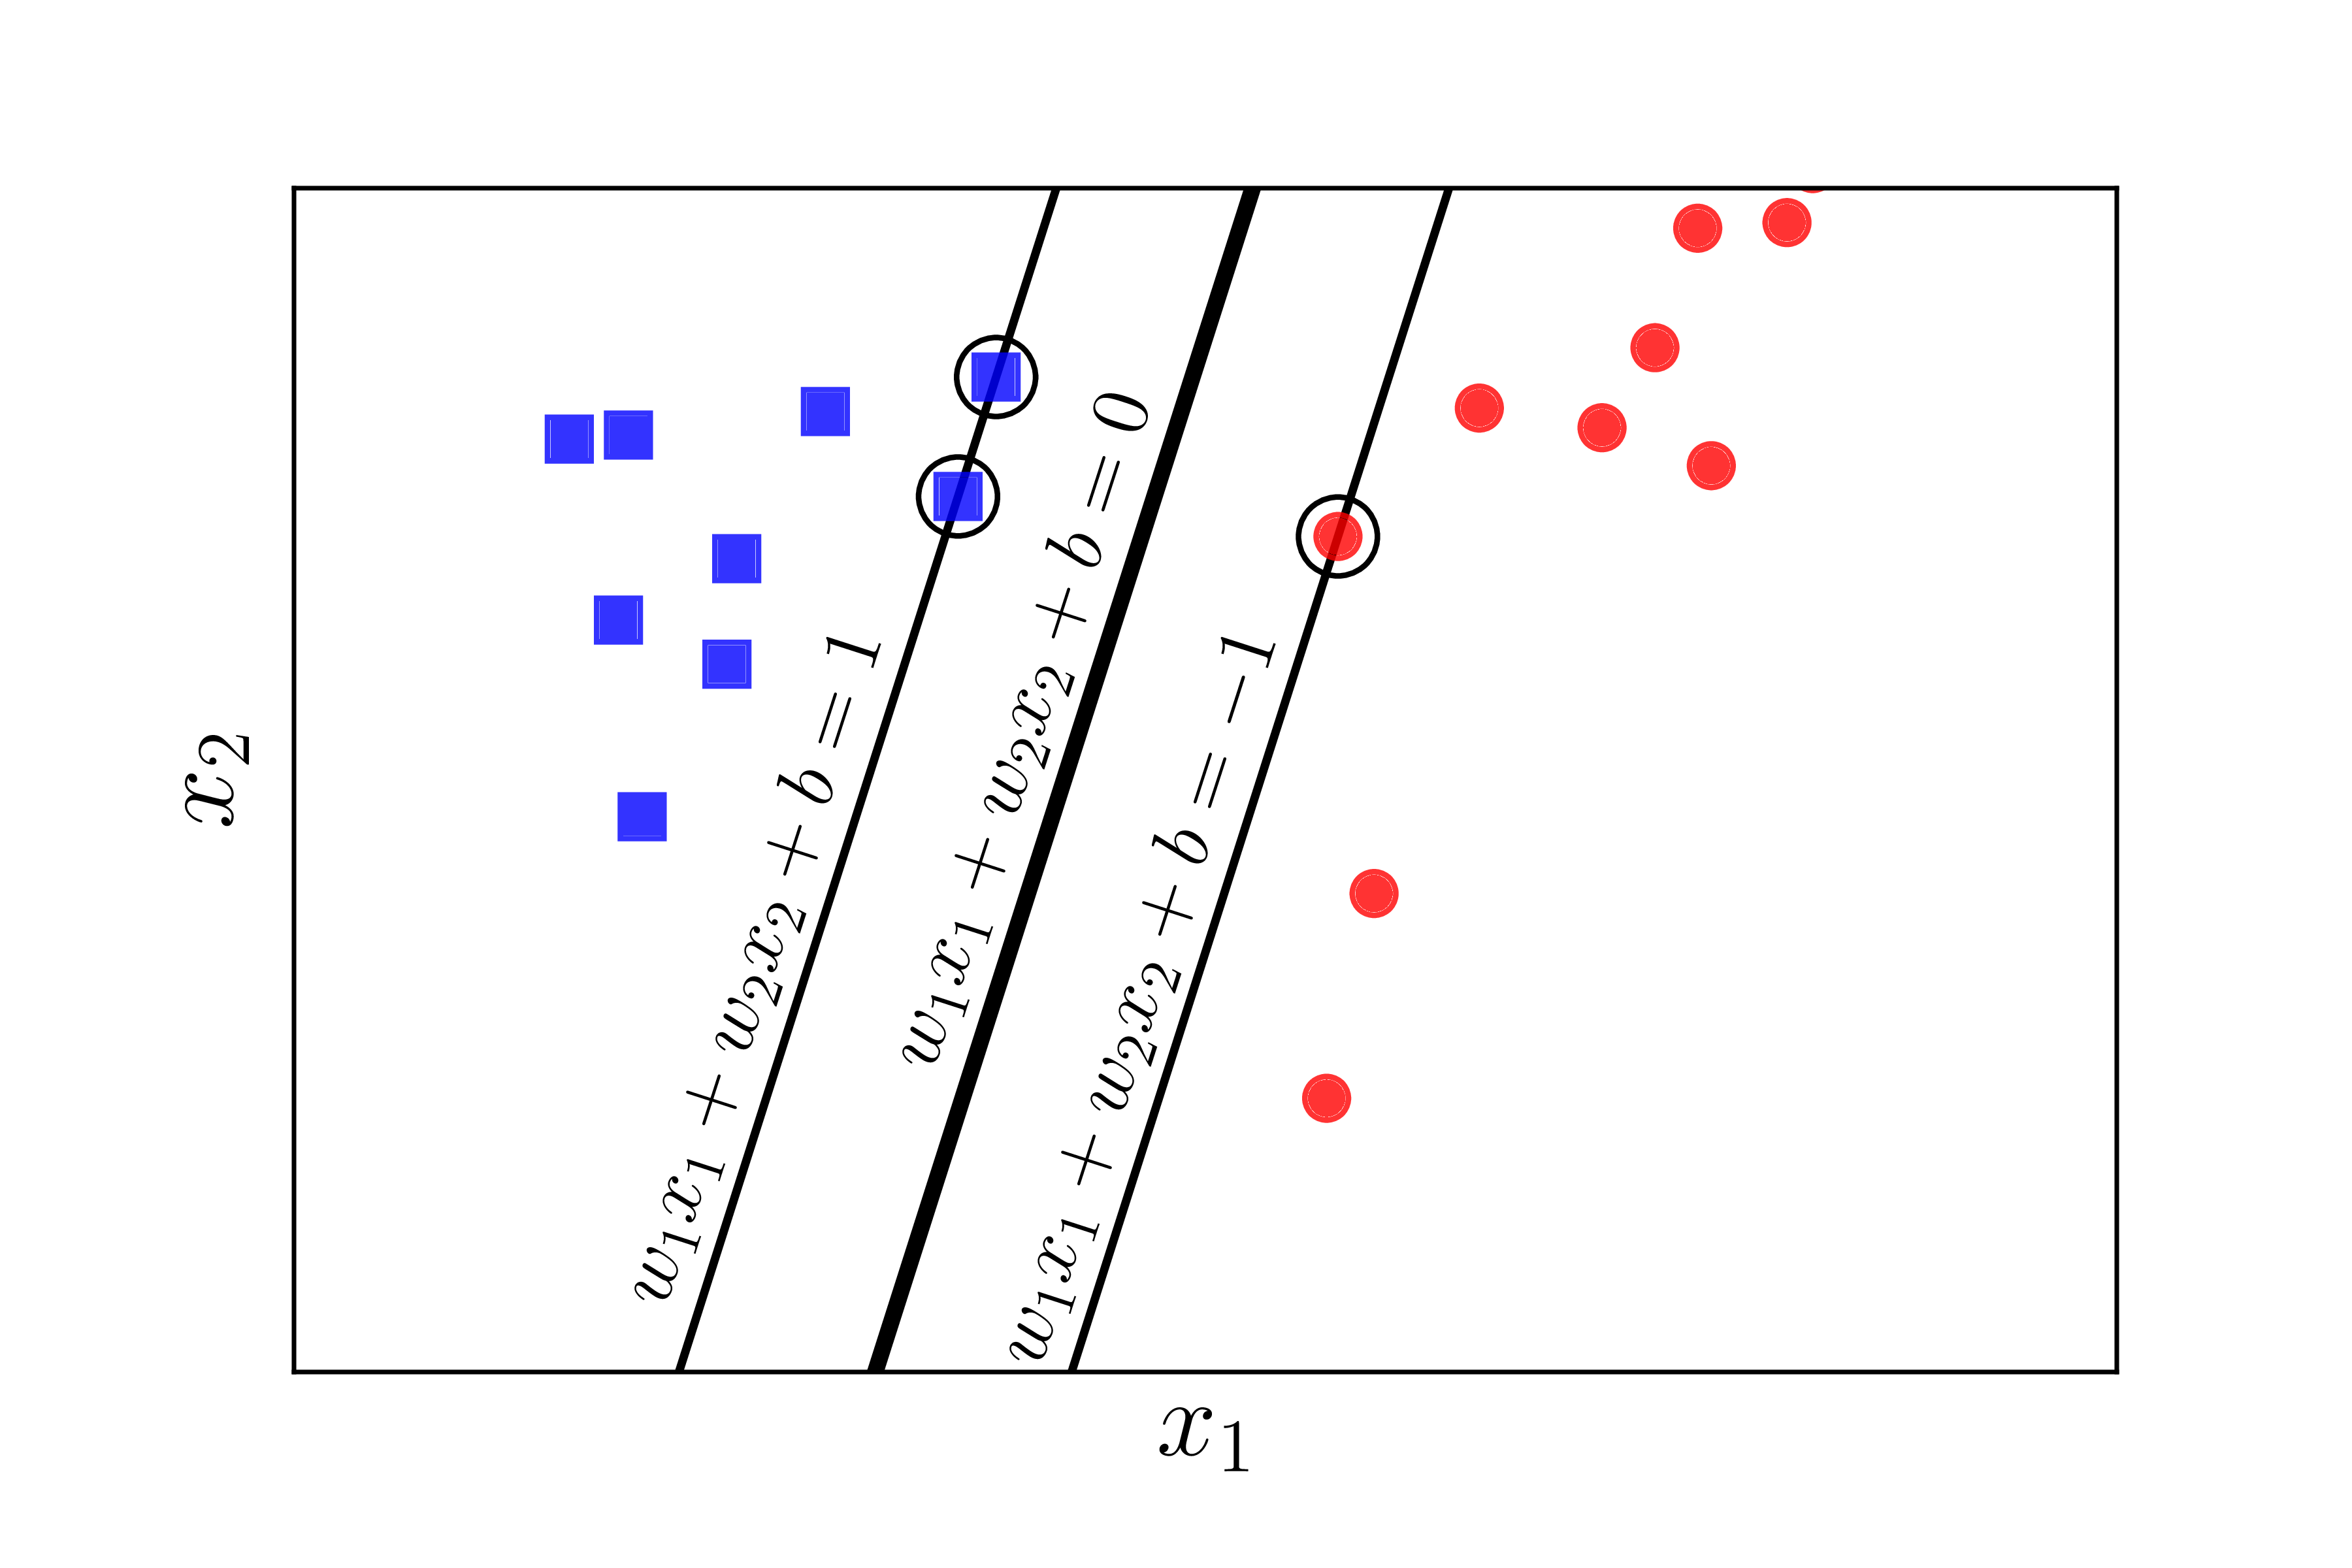
\includegraphics[width=1\linewidth]{Chapters/items/svm3.jpg}
        \label{fig:svm}
    \end{subfigure}
    \caption{Mô tả cơ chế phân loại của SVM}
\end{figure}

\newpage
\subsection{Nhận diện khuôn mặt và tiến hành điểm danh}
Khi hệ thống đã thực hiện huấn luyện xong các mô hình học sâu, tôi tiến hành thử nghiệm với một số ảnh có các khuôn mặt đã
đăng ký và chưa đăng ký.

Hệ thống sẽ dò tìm các khuôn mặt trong ảnh, sau đó thực hiện việc mã hóa các khuôn mặt này thành các vector đặc trưng
rồi đưa vào các mô hình phân loại đã được huấn luyện.

Kết quả cuối cùng hệ thống sẽ đưa ra hình ảnh các khuôn mặt và kém theo các tên của khuôn mặt đó
nếu khuôn mặt này đã được đăng ký, ngược lại hệ thống sẽ đưa ra "unknown face" nếu khuôn mặt này
chưa xuất hiện trong tập dữ liệu đã đăng ký

\begin{figure}
    \begin{subfigure}{1\textwidth}
        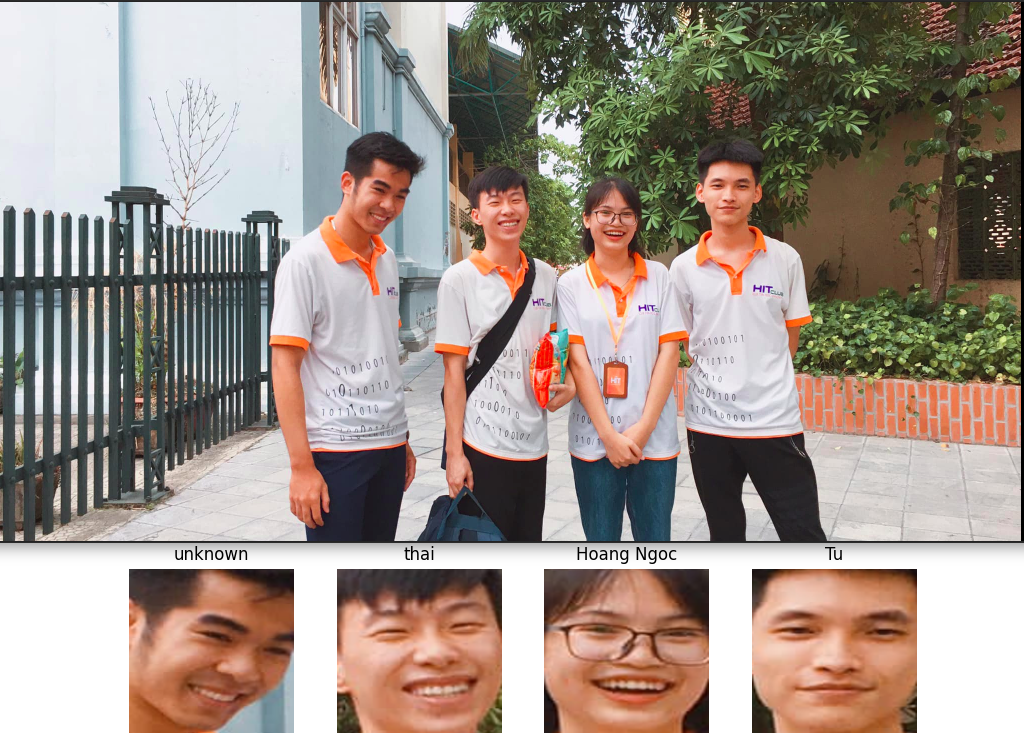
\includegraphics[width=1\linewidth]{Chapters/items/recog.png}
        \label{fig:recog}
    \end{subfigure}
    \caption{Hệ thống tiến hành điểm danh}
\end{figure}
\newpage
\subsection{Kết quả thử nghiệm}
\subsubsection{Độ chính xác của mô hình facenet}


\begin{figure}
    \begin{subfigure}{1\textwidth}
        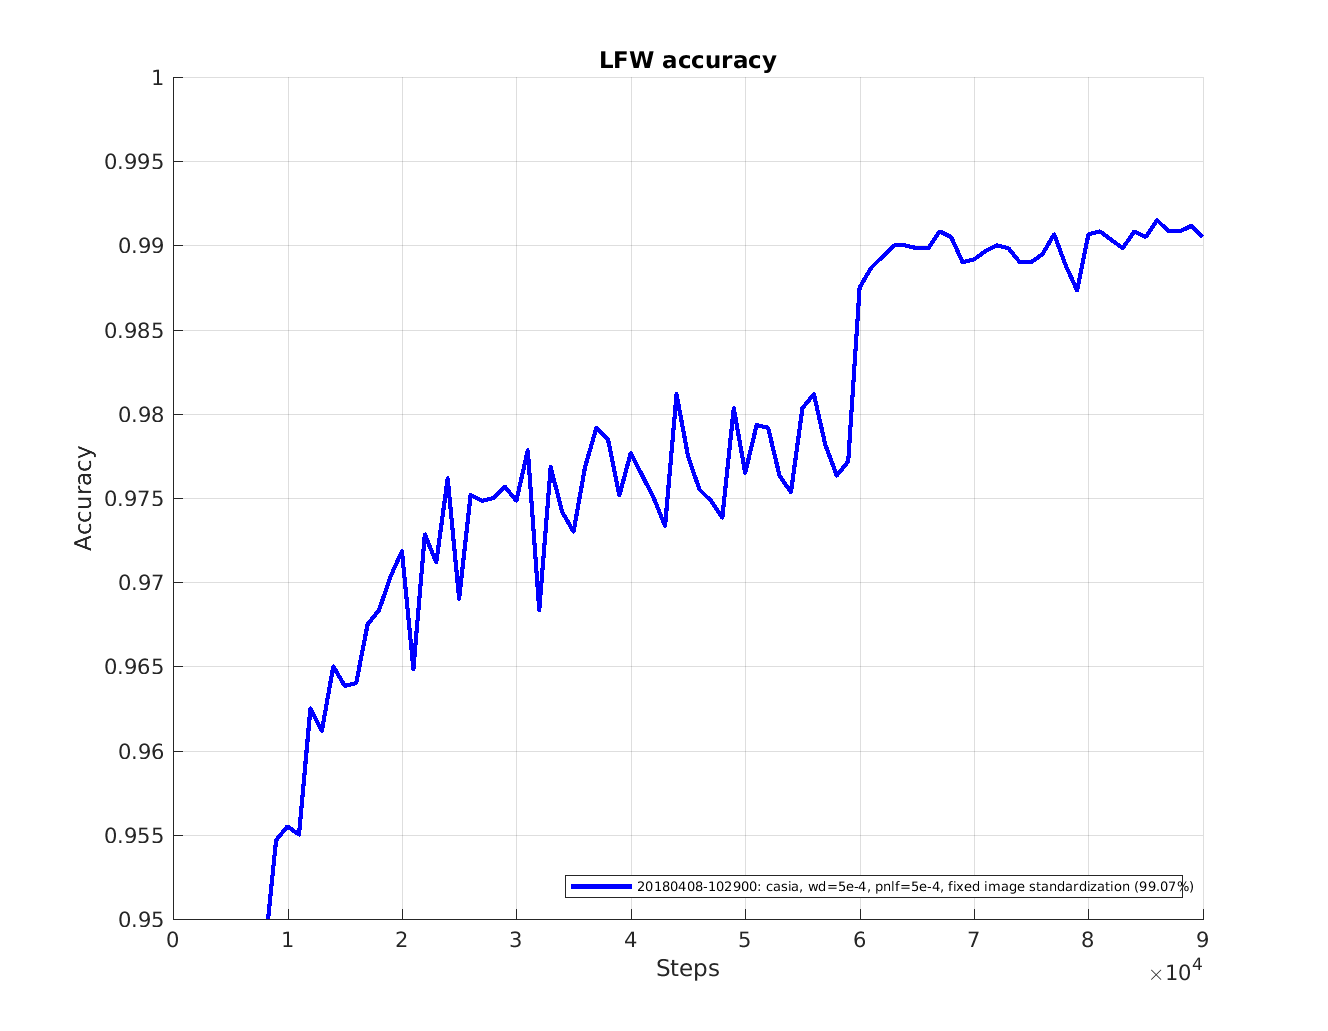
\includegraphics[width=1\linewidth]{Chapters/items/accuracy.png}
        \label{fig:accuracy}
    \end{subfigure}
    \caption{Độ chính xác trên tập dữ liệu LFW}
\end{figure}

Ở đây có thể thấy rằng ngay cả khi độ chính xác trong lần đánh giá cuối cùng
là 0,9965 thì độ chính xác trung bình cho 10 lần đánh giá cuối cùng thấp
hơn một chút (0,9950), có lẽ gần với những gì người ta có thể mong đợi khi
tái tạo kết quả. Mức trung bình có lẽ là một số liệu tốt hơn để sử dụng khi
so sánh các cài đặt siêu tham số khác nhau.

\begin{figure}
    \begin{subfigure}{1.\textwidth}
        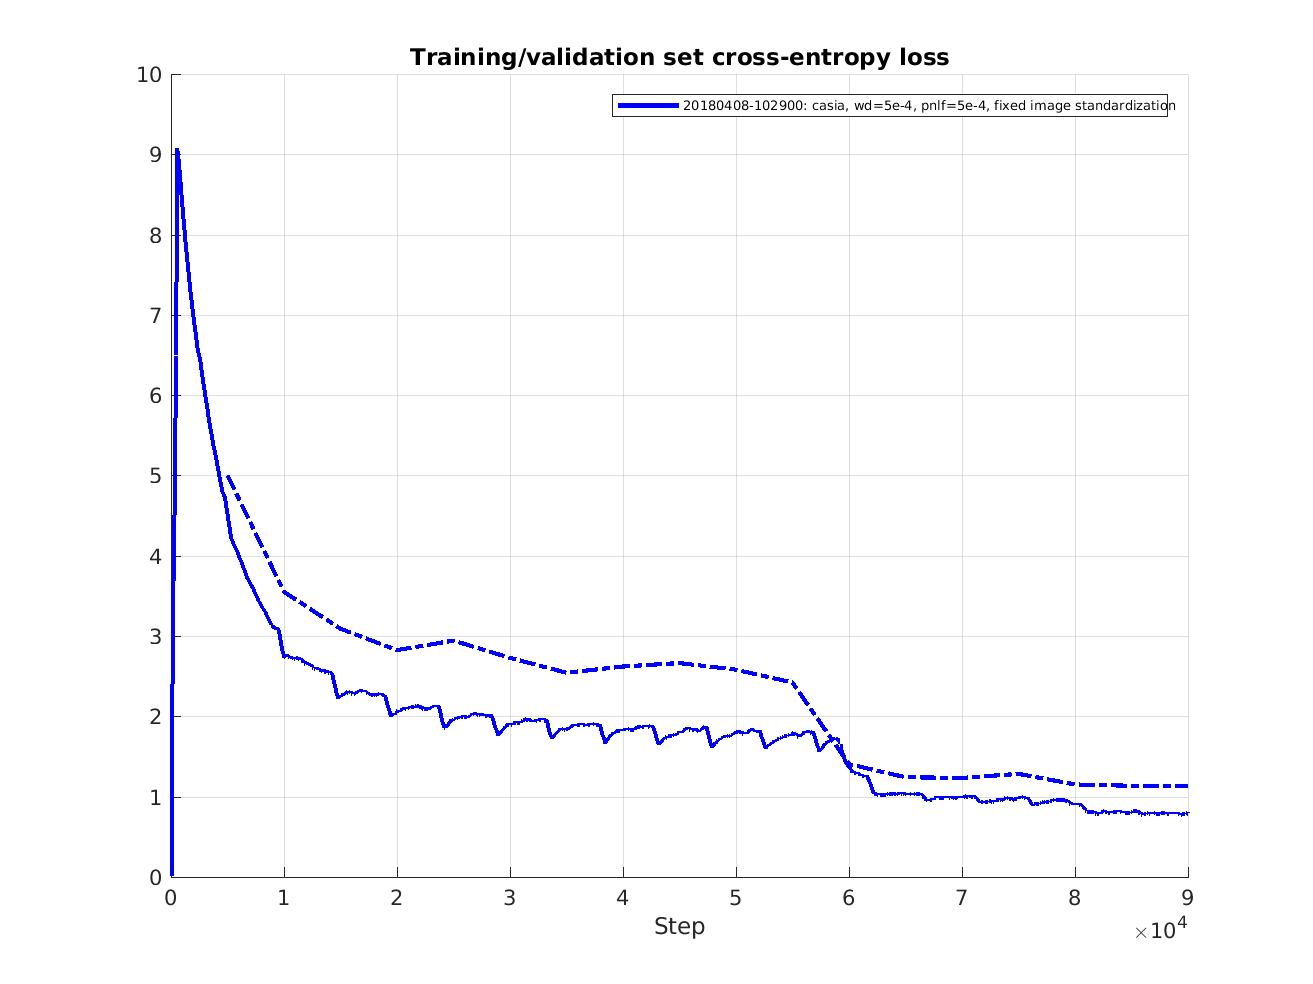
\includegraphics[width=1\linewidth]{Chapters/items/validate.png}
        \label{fig:validate}
    \end{subfigure}
    \caption{Đánh giá mất mát bằng Entropy chéo}
\end{figure}

\newpage
Hình này cho thấy sự mất mát entropy chéo trong quá trình huấn luyện (đường liền nét) và xác nhận (đường đứt nét). Bộ xác nhận bao gồm khoảng 20000 hình ảnh và đánh giá được thực hiện sau mỗi 5 kỷ nguyên. Entropy chéo trong quá trình đào tạo được ghi lại ở mỗi bước đào tạo nhưng đã được lọc bằng bộ lọc trung bình trượt trên 500 bước. Từ điều này, rõ ràng là mô hình có lợi hơn một chút vì vậy có thể tốt nếu thử nghiệm thêm một chút với xác suất phân rã trọng lượng L2 và xác suất bỏ học.

\newpage
\subsubsection{Hiệu suất của hệ thống}

Khi sử dụng các phương pháp đo độ chính xác trên dữ liệu thức tế mà tôi tự thu thập từ
những người bạn, sinh viên trong khoa, trường. Thì độ chính xác đo được là 96.4\%

\begin{figure}
    \begin{subfigure}{0.6\textwidth}
        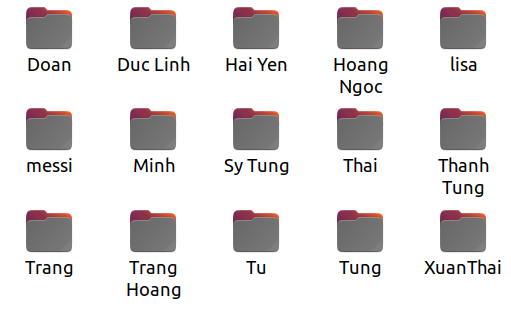
\includegraphics[width=1.0\linewidth]{Chapters/items/dataset.png}
        \label{fig:dataset}
    \end{subfigure}
    \caption{Dữ liệu tự thu thập}
\end{figure}
